\newpage
\section{Polarización del punto Q}
\midTitle{red}{Parte analítica}{}
\sangria{En este trabajo implementamos un transistor JFET en configuración fuente común, para aplicar el modelo MES, en esta oportunidad implementamos el modelo con autopolarización.
Nuestros datos iniciales fueron $V_{DD}= 12V$ $R_G=1M\Omega$, además contábamos también con los datos del punto Q ya predefinidos $I_{DQ}=\frac{I_{DSS}}{2}$ y $V_{DSQ}=\frac{V_{DD}}{2}$}
\sangria{Primero relevamos la curva de $I_{DSS}$, para luego calcular $R_S$ $R_D$, la curva relevada fue la siguiente.}

\midTitle{blue}{Mediciones de $I_{DSS}$ Obtenidas}{}

\begin{center}
\setlength{\tabcolsep}{4pt}
\captionof{table}{Mediciones de $I_{DSS}$ en función de $V_{DS}$.}
\begin{tabular}{|
>{\columncolor[HTML]{FFCCC9}}c |
c | c |}
\hline
\rowcolor[HTML]{FFFFC7}
\textbf{$V_{DS}$ (V)} & \textbf{$I_{DSS}$ (mA)} & \textbf{Diferencia (\%)} \\ \hline
0.200 & 2.112 & - \\ \hline
0.440 & 4.530 & 114.5 \\ \hline
0.600 & 5.500 & 21.4 \\ \hline
0.820 & 6.050 & 10.0 \\ \hline
1.015 & 6.390 & 5.6 \\ \hline
1.235 & 6.560 & 2.7 \\ \hline
1.402 & 6.650 & 1.4 \\ \hline
1.650 & 6.742 & 1.4 \\ \hline
1.815 & 6.787 & 0.7 \\ \hline
2.020 & 6.834 & 0.7 \\ \hline
2.200 & 6.853 & 0.3 \\ \hline
2.450 & 6.893 & 0.6 \\ \hline
2.609 & 6.913 & 0.3 \\ \hline
2.830 & 6.942 & 0.4 \\ \hline
\end{tabular}
\end{center}

\begin{figure}[H]

   \centering
    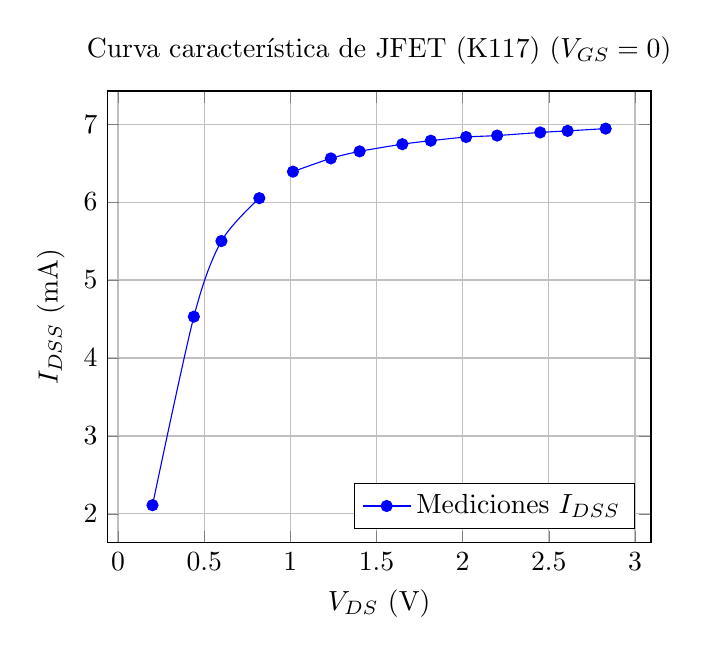
\begin{tikzpicture}
    \begin{axis}[
        title={Curva característica de JFET (K117) ($V_{GS} = 0$)}, % Título del gráfico
        xlabel={$V_{DS}$ (V)},          % Etiqueta eje X
        ylabel={$I_{DSS}$ (mA)},        % Etiqueta eje Y
        grid=major,                   % Grilla principal
        legend pos=south east,        % Posición de la leyenda (esquina inf. derecha)
        width=0.7\textwidth,          % Ancho del gráfico
    ]

    \addplot [
        smooth,
        mark=*,
        blue,
    ]
    coordinates {
        (0.200, 2.112)
        (0.440, 4.530)
        (0.600, 5.500)
        (0.820, 6.050)

        (1.015, 6.390)
        (1.235, 6.560)
        (1.402, 6.650)
        (1.650, 6.742)
        (1.815, 6.787)
        (2.020, 6.834)
        (2.200, 6.853)
        (2.450, 6.893)
        (2.609, 6.913)
        (2.830, 6.942)
    };
\addlegendentry{Mediciones $I_{DSS}$}

    \end{axis}
    \end{tikzpicture}
    \caption{Curva de salida $I_D = f(V_{DS})$ para $V_{GS} = 0$.}
    \label{fig:curva_jfet}
\end{figure}
\newpage
\subsection{Cálculos del punto Q}

\begin{figure}[!ht]
\centering
\resizebox{0.3\textwidth}{!}{%
\begin{circuitikz}
\tikzstyle{every node}=[font=\normalsize]
\draw (-11.25,25.75) to[short] (-8.75,25.75);
\draw (-11.25,25.75) to[R] (-11.25,23.25);
\draw (-8.75,25.75) to[battery ] (-8.75,23.25);
\draw (-11.25,23.25) to[short] (-11.75,23.25);
\draw [->, >=Stealth] (-12.75,22.75) .. controls (-11.75,22.75) and (-12.25,22.75) .. (-11.75,22.75) ;
\draw (-8.75,23.25) to[short] (-8.75,20.75);
\draw (-12.75,20.75) to[short] (-8.75,20.75);
\draw (-11.75,23.25) to[short] (-11.75,22.25);
\draw (-11.75,22.25) to[short] (-11.25,22.25);
\draw (-12.75,22.75) to[R] (-12.75,20.75);
\draw (-11.25,22.25) to[R] (-11.25,20.75);
\node [font=\normalsize] at (-13.5,21.75) {$R_{G}$};
\node [font=\normalsize] at (-11.75,21.75) {$R_{S}$};
\node [font=\normalsize] at (-12,24.75) {$R_{D}$};
\node [font=\normalsize] at (-8.5,25) {+};
\node [font=\normalsize] at (-8.5,24) {-};
\node [font=\normalsize] at (-9.5,24.5) {$V_{DD}$};
\draw (-8.75,20.75) to (-8.75,20.25) node[ground]{};
\end{circuitikz}
}%

\label{fig:my_label}
\end{figure}

\sangria{Una vez revelada la curva, el valor de $I_{DSS}$ se extrajo a partir de las diferencias porcentuales del mismo valor, el valor elegido fue: $I_{DSS} = 6,650\text{ mA}$, ya que la diferencia porcentual con el valor anterior fue del $1.4\%$, el valor de tensión en este punto se denomina $V_{GSoff}$ y es de $V_{GSoff}=-1,402\text{ V}$}

$$I_{DQ}=\frac{I_{DSS}}{2} \quad \rightarrow \quad I_{DQ}=\frac{6,650\text{ mA}}{2} \quad \rightarrow \quad I_{DQ}=3,325\text{ mA}$$
$$V_{DSQ}=\frac{V_{DD}}{2} \quad \rightarrow \quad V_{DSQ}=\frac{12\text{ V}}{2} \quad \rightarrow \quad V_{DSQ}=6\text{ V}$$

\sangria{El siguiente paso fue calcular las resistencias para situar el punto Q, para esto primero obtenemos el valor de $V_{GS}$ para luego obtener $R_S$ y finalmente
obtenemos $R_D$. Las ecuaciones de las cuales obtenemos estos valores son las siguientes:}


$$i_{D}=I_{DSS} \cdot \left(1-\frac{V_{GS}}{V_{GSoff}}\right)^2$$
$$V_{GS}=-i_{D} \cdot R_{S}$$
$$V_{DD}=i_{D} \cdot (R_{S} + R_{D})+V_{DS}$$

\sangria{De la primera ecuación despejamos $V_{GS}$, como nos encontramos en el punto Q, podemos sustituir $i_D$ por $I_{DQ}$ y queda:}


$$V_{GS}=\left(\sqrt{\frac{I_{DQ}}{I_{DSS}}}-1\right) \cdot (-V_{GSoff}) \quad \rightarrow \quad V_{GS}=\left(\sqrt{\frac{I_{DSS}/2}{I_{DSS}}}-1\right) \cdot (1,402\text{ V}) \quad \rightarrow \quad V_{GS}=-0,4106\text{ V}$$


\sangria{Con este dato podemos obtener $R_S$ a partir de la segunda ecuación:}

$$R_S=\left|\frac{-V_{GS}}{I_{DQ}}\right|
= \left|\frac{-(-0,4106\text{ V})}{3,325\text{ mA}}\right| = 123,48\ \Omega \quad \xrightarrow{\text{Normalizado}} \quad R_S=120\ \Omega$$

\sangria{Ya con este valor podemos calcular $R_D$ a partir de la 3ra ecuación.
Para el cálculo de $R_D$ se utiliza el valor no normalizado de $R_S$ para mayor precisión:}


$$R_D=-R_S +\frac{V_{DD}-V_{DSQ}}{I_{DQ}} = -123,48\ \Omega +\frac{12\text{ V}-6\text{ V}}{3,325\text{ mA}} = 1681,51\ \Omega \quad \xrightarrow{\text{Normalizado}} \quad R_D=1,8\text{ k}\Omega$$


\begin{table}[H]
\caption{Valores del punto Q}
\label{table2}
\resizebox{\textwidth}{!}{%
\begin{tabular}{|
>{\columncolor[HTML]{FFCCC9}}c |cc|}
\hline
\cellcolor[HTML]{FFFC9E}\textbf{Parámetro} &
  \multicolumn{1}{c|}{\cellcolor[HTML]{FFFC9E}\textbf{Valor Calculado (No normalizado)}} &
  \cellcolor[HTML]{FFFC9E}\textbf{Valor Normalizado (Comercial)} \\ \hline
$V_{GSQ}$ & \multicolumn{1}{c|}{$-0.4106\text{ V}$} & --- \\ \hline
$I_{DQ}$  & \multicolumn{1}{c|}{$3.325\text{ mA}$}  & --- \\ \hline
$V_{DSQ}$ & \multicolumn{1}{c|}{$6\text{ V}$}       & --- \\ \hline
$R_S$     & \multicolumn{1}{c|}{$123.48\ \Omega$}   & $120\ \Omega$         \\ \hline
$R_D$     & \multicolumn{1}{c|}{$1681.51\ \Omega$}  & $1.8\ \text{k}\Omega$ \\ \hline
\end{tabular}%
}
\end{table}

\subsection{Implementación circuito carga pasiva}
\midTitle{red}{Parte práctica}{}
\sangria{Cuando implementamos el circuito con un transistor JFET K117 y medimos, tuvimos que hacer un cambio en $R_S$, ya que la polarización no daba de la manera correcta, fuimos bajando el valor hasta llegar a $80\ \Omega$, con ese valor la polarización nos dio los siguientes valores:}
\sangria{Para medir $I_{DQ}$ dividimos la tensión medida en la resistencia $R_D$, dividido el valor de esta ($1,8\text{ k}\Omega$), el resultado fue de $I_{DQ}=3,144\text{ mA}$ y
la $V_{DS}=6,12\text{ V}$}



\begin{table}[H]
\caption{Valores del punto Q: Comparación Calculados vs. Medidos}
% \label{} % ¡Ponle una etiqueta (label) única!
\resizebox{\textwidth}{!})} & \textbf{Valor Medido} & \textbf{Diferencia (\%)} \\ \hline

% Datos de la fila VDSQ
$V_{DSQ}$ & 6 V & $[5.4\text{ V} ;
6.6\text{ V}]$ & 6.12 V & 2.0\% \\ \hline

% Datos de la fila IDQ
$I_{DQ}$ & 3.325 mA & $[2.99\text{ mA} ;
3.66\text{ mA}]$ & 3.144 mA & 5.4\% \\ \hline
\end{tabular}%
}
\end{table}


\midTitle{teal}{Resultados}{}
\sangria{Al comparar los resultados obtenidos en la ``Parte analítica`` con los medidos en la ``Parte práctica``, se observa una muy buena correlación entre el modelo teórico y el comportamiento real del circuito.
Como se detalla en la \textbf{Tabla 3}, el valor medido de $V_{DSQ}$ ($6.12\text{ V}$) presentó una diferencia porcentual de solo \textbf{2.0\%} con respecto al valor calculado de $6\text{ V}$.}

\sangria{Por su parte, la corriente $I_{DQ}$ medida ($3.144\text{ mA}$) tuvo un desvío del \textbf{5.4\%} frente al valor teórico de $3.325\text{ mA}$.
Esta diferencia es atribuible a la discrepancia encontrada durante la implementación práctica.
El valor calculado para la resistencia $R_S$ fue de $123.48\ \Omega$ (normalizado a $120\ \Omega$), pero en el laboratorio fue necesario ajustar este valor a $\mathbf{80,2}\ \Omega$ para lograr la polarización correcta, tal como se describe en el texto de la parte práctica.}

\sangria{Este ajuste en $R_S$ es la principal fuente del error porcentual en $I_{DQ}$.
A pesar de esto, una diferencia del 5.4\% se considera aceptable y valida el modelo analítico como una herramienta de diseño eficaz, demostrando que los cálculos teóricos del punto Q sirvieron como una excelente aproximación para la implementación física.}
